\section{Implementation}
\label{sec:implementation}

In this section we present details about our implementation, including a
prototype framework and three non-trivial wide-area streaming applications.
\sysname{} is implemented in Rust and open-source on Github.\footnote{Url elided
  for anonymity.}

\subsection{Framework}
\label{sec:framework}

While our proposed APIs are general and not language specific, we chose a safe
language, Rust, for the core framework for the following reasons. First, Rust's
memory safety guarantee can ensure applications running continously for an
extended period of time. Besides, the zero-cost abstraction removes the
possibilities of tail latencies caused by uncoordinated garbage
collection~\cite{maas2016taurus}. In addition, we rely on Rust's type system to
enforce the type match on \texttt{maybe} operations.

\begin{sloppypar}
All operators implement the \texttt{Stream} trait which has an associate type
\texttt{Item} and a core function \texttt{next} that returns
\texttt{Datum}. Each datum is either an item with the \texttt{Stream::Item} or
an \texttt{Error} that the operator use to communicate with the runtime
scheduler. The concrete form of \texttt{maybe} API is almost an direct
translation of the API specification. While our API specification
in~\autoref{tab:operators} uses a vector for knobs, our Rust implementation is
more general: any type (including vector) that implements \texttt{IntoKnob}
trait can be used as the knob.
\end{sloppypar}

\begin{lstlisting}
pub trait Stream {
    type Item;
    fn next(&mut self) -> Datum<Self::Item, Error>;

    fn maybe<K, F>(self, opts: K, f: F) -> Maybe<Self, F>
        where Self: Sized,
                K: IntoKnob,
                F: FnMut(K::Item, Self::Item) -> Self::Item {

         // omitted
    }
}

pub trait IntoKnob {
    fn into_knob(self) -> Knob;
}
\end{lstlisting}

Developers can directly use the above API with user-defined functions. The
snippet below shows how a quantization degradation can be implemented with our
API. First, a vector of values is converted into a stream object. Then a
\texttt{maybe} operator with a knob value (2 or 3) and a function that performs
an interger division (quantization). Function \texttt{collect} will run this
stream and hold the output in a vector. Depending on the degradation level, the
output stream could either be [1, 2, 3, 4], [0, 1, 1, 2], or [0, 0, 1, 1].

\begin{lstlisting}
let quantized_stream = vec![1, 2, 3, 4]
    .into_stream()
    .maybe(vec![2, 3],
             |knob, p| p / knob);
    .collect();
\end{lstlisting}

We've also extended the basic API for common operations. As we are building
video processing applications, we implemented a specialized
\texttt{maybe\_downsample} operator can that wraps \texttt{downsample} function
internally.

\begin{lstlisting}
fn downsample(res: (usize, usize), image: Mat) -> Mat {

    //  omitted

}
\end{lstlisting}

Applications built with \sysname{} runs as a single process. The entire
processing pipeline is often specified in a single main file. The execution mode
(profiling, runtime as client or runtime as server) is configured with command
line arguments or environment variables. Our deployment manager is currently a
shell script using Docker container.

\subsection{Building \sysname{} Applications}
\label{sec:build-appl}

Using \sysname{}, we've built three applications: pedestrian detection
surveillance, an augmented reality and a distributed Top-k (\autoref{fig:apps}).
\autoref{tab:apps} summarizes the application specific part: knobs, utility
function and dataset

\begin{table*}
  \small
  \centering
  \begin{tabular}{|c|c|c|c|}
    \hline
    Application & Knobs & Utility & Dataset \\
    \hline
    Pedestrian Detection & resolution, framerate, quantizer
                        & F1 score & MOT16-04 (training), MOT16-03 (testing) \\
    \hline
    Augmented Reality & resolution, framerate, quantizer
                        & F1 score & Video clips of office (training), home (testing) \\
    \hline
    Top-K & head (N), local threshold (T) & Kendall's W & sec.gov access log
                                                          (4 days training, 12 days testing)  \\
    \hline
  \end{tabular}
  \caption{\sysname{} Applications}
  \label{tab:apps}
\end{table*}

\begin{figure*}
  \centering
  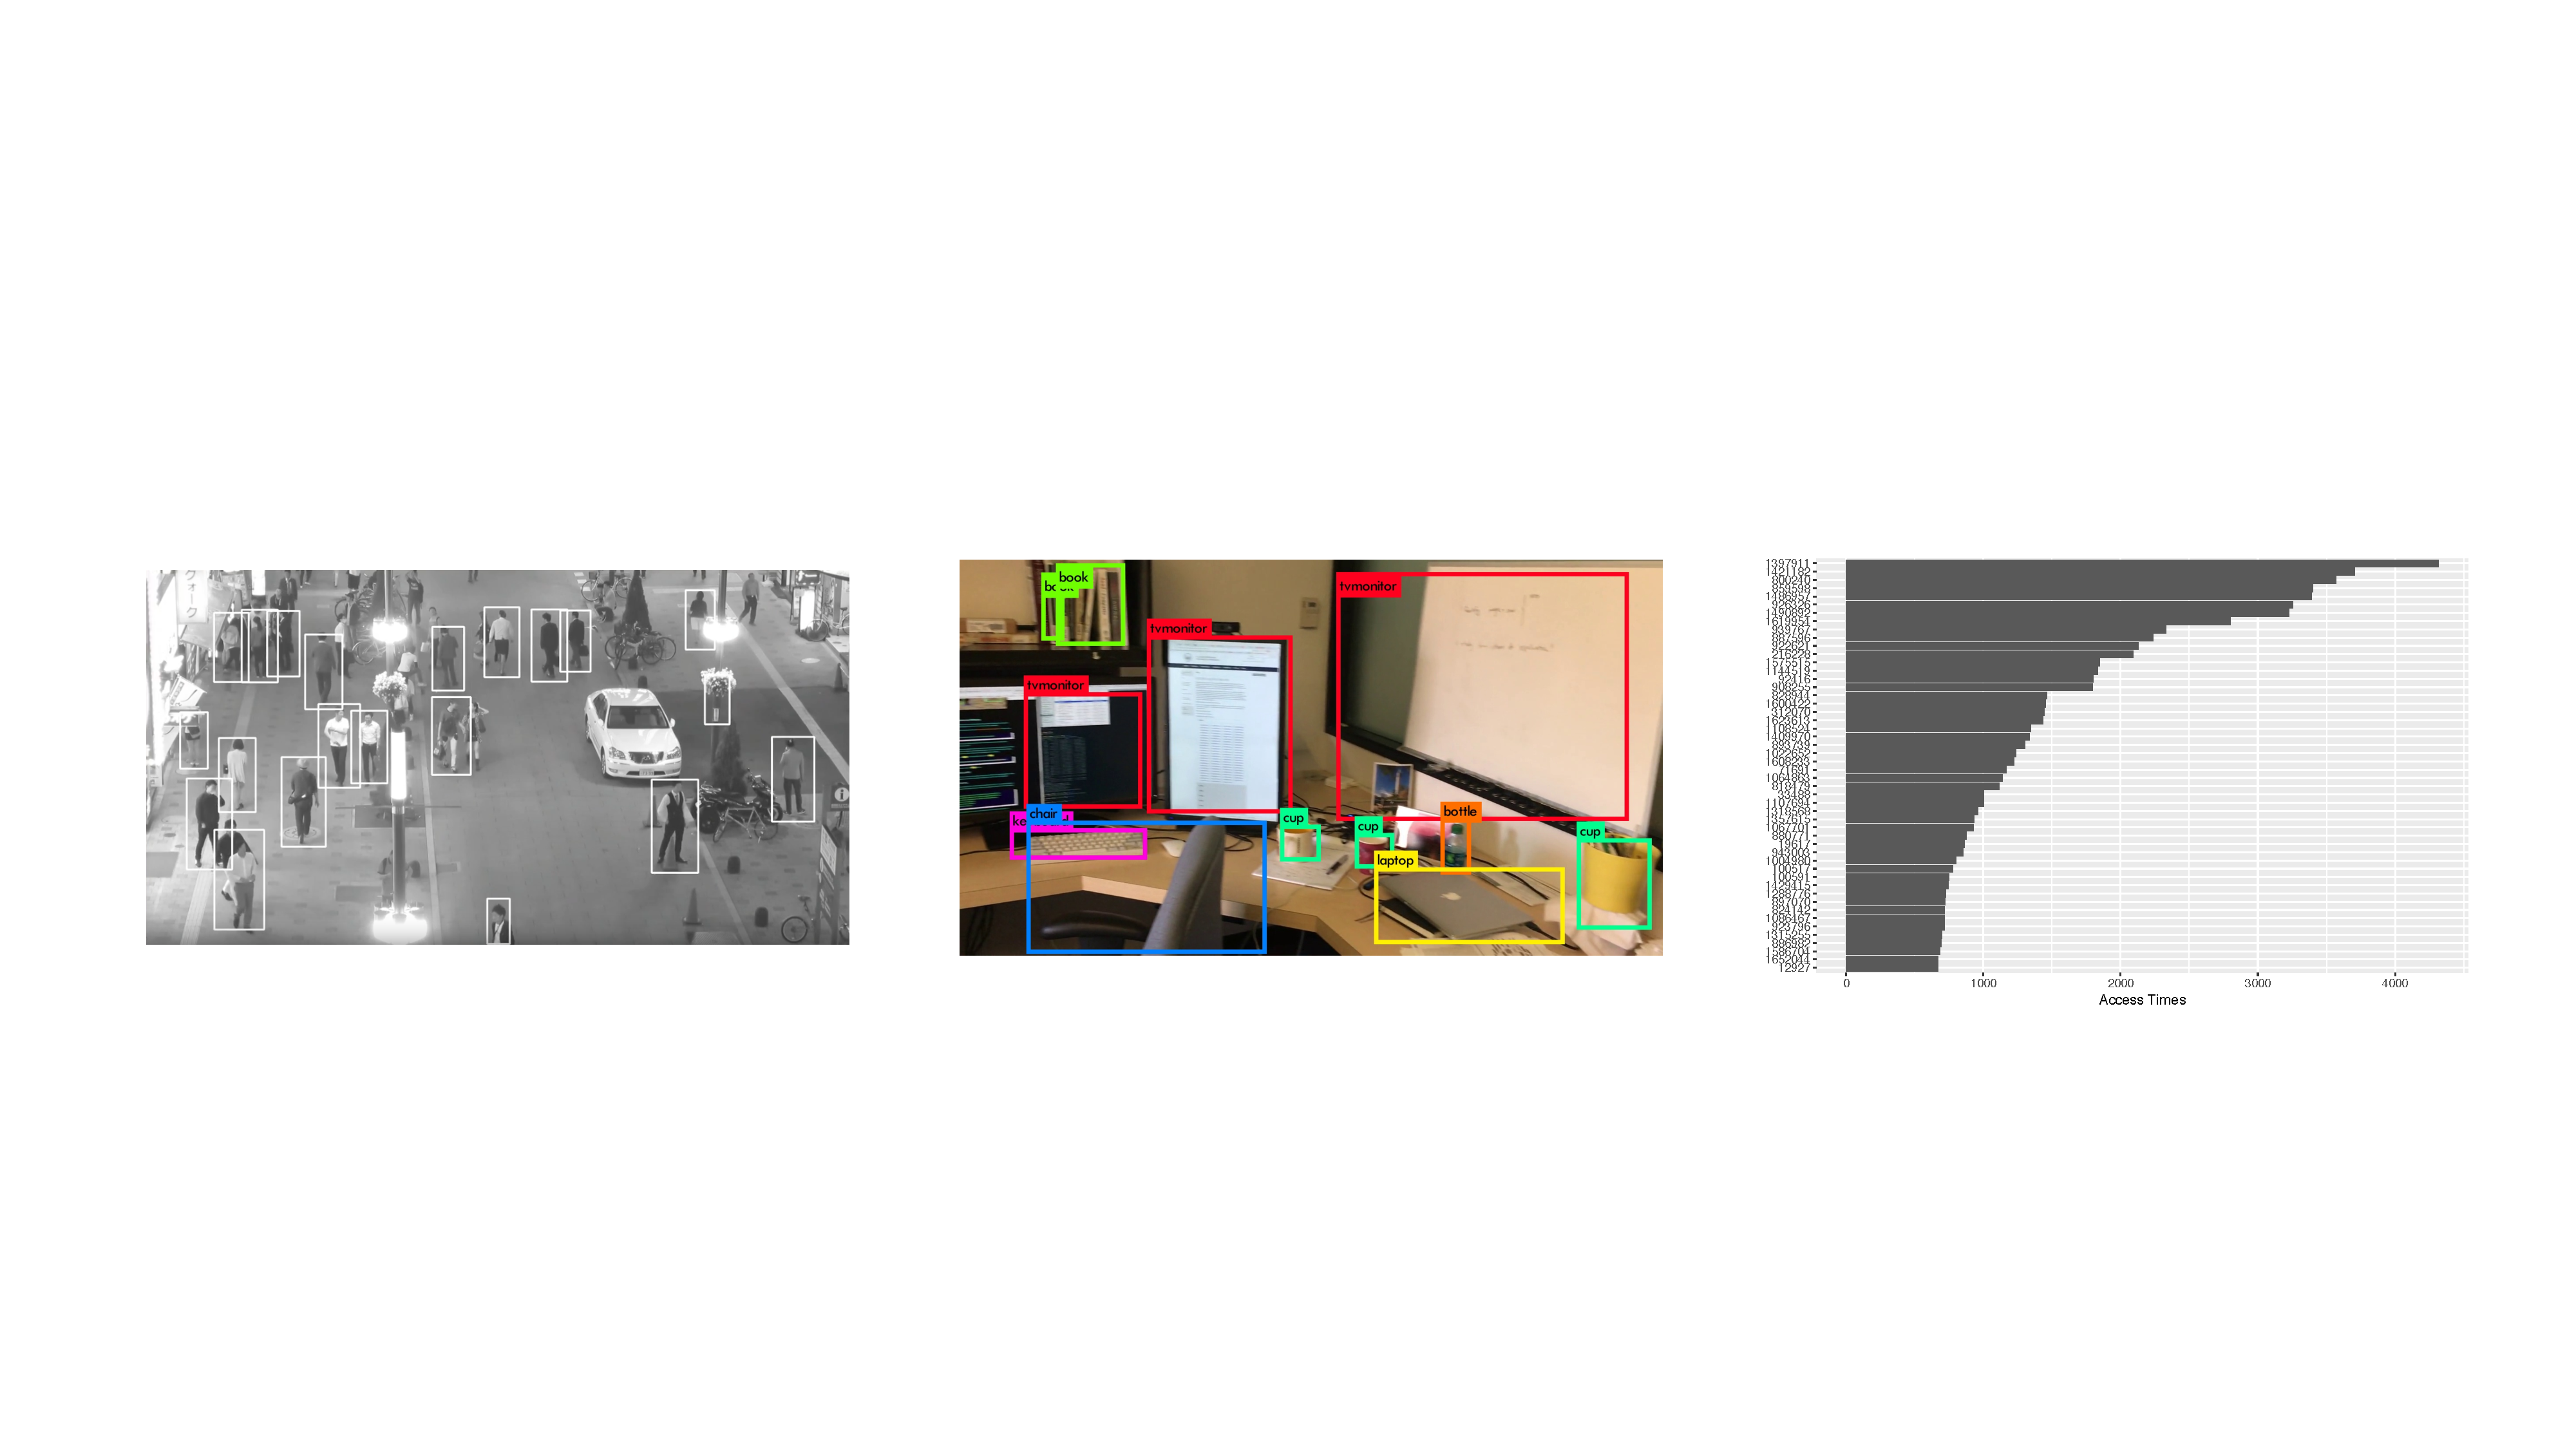
\includegraphics[width=.95\textwidth]{figures/apps.pdf}
  \caption{\sysname{} applications}
  \label{fig:apps}
\end{figure*}

\para{Pedestrian Detection:} This application analyzes video streams from
installed CCTV cameras and detect pedestrians inside. The detection result is a
list of bounding boxes representing pedestrian's relative location within the
view. Variant of this application can be used for safety monitoring, anomaly
detection or waiting line counting.

We implement most image-related operations with OpenCV
3.1~\cite{opencvlibrary}. Pedestrians are detected using histogram of oriented
gradients (HOG)~\cite{dalal2005histograms} with the default linear SVM
classifier. To ensure real-time processing of frames, GPU-accelerated
implementation is used in favor of the CPU-based implementation.

For video encoding, H.264 scheme is chosen for its prevalence in existing
systems. Our implemenation is based on GStreamer~\cite{gstreamer}, using
\texttt{x264enc} plugin. To integrate with \sysname{}, we first create a
pipeline that exposes \texttt{appsrc} (to feed raw image data) and
\texttt{appsink} (to get encoded bytes). The GStreamer main loop is managed in a
separate thread and \sysname{} communicates with it via Rust's channel. The
\texttt{x264enc} is configured with \texttt{zerolatency} present and runs using
four threads. It uses constant quality encoding and the quantizer is exported as
a parameter that can be tuned.

This application has three degradation operations: reducing image resolution,
dropping frame rate or lower video encoding quality.

The detection returns a list of bounding boxes; it's compared against a
reference result (either the groundtruth or the one without degradation). A
successful detection is defined when the intersection over union (IOU) is
greater than 50\%~\cite{everingham2010pascal}. For the utility function, we use
F1 score (\%), the harmonic mean of precision and
recall~\cite{Rijsbergen:1979:IR:539927}.

\para{Augmented Reality:} We target at mobile augmented reality applications
which offload the heavy computation to resources elsewhere. Although local
computation is gaining attraction~\cite{satyanarayanan2009case, zhang2015cloud},
wireless communication link is also susceptible to capacity variation.

We use a similar setup as the pedestrian detection application except the actual
function that analyzes the stream. To recognize objects, we use a a pre-trained
neural network~\cite{darknet13} that's trained with
Imagenet~\cite{krizhevsky2012imagenet}. Similar to our first application,
GPU-accelerated implementation is use in favor for real-time processing.

The utility function here is more strict than the pedestrian detection:
true-positive depends not only on IOU criteria, but also on the type of objects
(a correct identification).

\para{Distributed Top-K:} Many distributed system monitoring applications
require to answer the ``top-k'' question~\cite{babcock2003distributed}, such as
the top-k most popular URLs or the top-k most access files. Naive methods of
transmitting all the raw log entries to the aggregation point is not feasible as
popular servers typically have millions of requests per second. Local worker
node can first perform a window-based transformation that generates data
summary, such as key-value pairs of \texttt{<item, count>}. However, even after
this operation, the data size could still be too large given most real-world
access patterns follow a long-tailed distribution. There is a
large-but-irrelevant tail that is unnecessary to send.

We consider two degradation operations that individual worker nodes can perform:
(1) a local Top-\texttt{N} operation that shortens the list first; (2) a local
threshold \texttt{T} that further filters small entries. Obviously, these two
operations are not orthognal to each other. Their impact on data size reduction
and quality degradation depends on the distribution of the actual data.

\begin{figure}
  \centering
  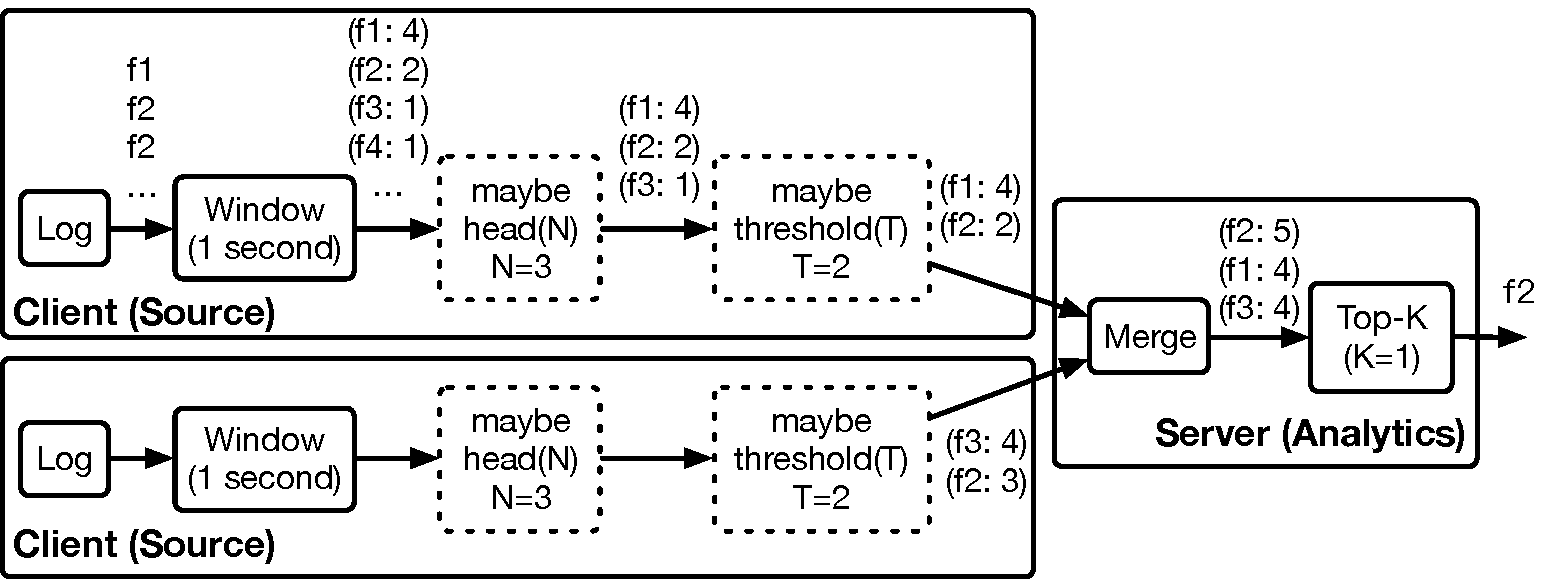
\includegraphics[width=\linewidth]{figures/topk.pdf}
  \caption{A distributed Top-K application has two tunable parameters: a local
    Top-N (N) and a local threshold (T).}
  \label{fig:topk}
\end{figure}


we use Kendall's W as the utility function here. It is a distance measure of the
concordance between two ranked list. The function outputs a statistic measure
ranging from 0 to 1, representing no agreement to complete aggrement,
respectively~\cite{abdi2007kendall}.

%%% Local Variables:
%%% mode: latex
%%% TeX-master: "sigcomm2017"
%%% End:
